\documentclass[a4paper,12pt]{report}
\usepackage[slovak,english]{babel}
\usepackage[T1]{fontenc}             
\usepackage[utf8]{inputenc}    
\usepackage{amsmath}
\usepackage{amssymb,amsfonts,amscd}
\usepackage{array,hhline}
\usepackage{makeidx}
\usepackage{fancyhdr}
\usepackage{graphicx}
\usepackage{listings}
    %%\usepackage{titlepage}
    %%\usepackage{multicol}
\usepackage{eurosym}
\usepackage{url,mathptmx} 
\usepackage[pdftex,unicode,bookmarks=false]{hyperref}




\renewcommand{\baselinestretch}{1.5}  % pre zvascenie riadkovania

\addtolength{\oddsidemargin}{-.5cm}
\addtolength{\evensidemargin}{-2.9cm}   
\addtolength{\topmargin}{0cm}
\addtolength{\textheight}{0pt}
\addtolength{\textwidth}{2.cm}
\addtolength{\textheight}{2.cm}
\newlength{\verbcorr}
\setlength{\verbcorr}{0ex}





\begin{document}
\selectlanguage{slovak}


\pagestyle{empty}
\pagenumbering{arabic}

\begin{titlepage}
\phantom.

\bigskip

\begin{center}
{\sc\LARGE Žilinská Univerzita v Žiline}
\medskip

{\sc\Large Fakulta riadenia a informatiky}

\vfill\vfill\vfill\vfill

{\sc\LARGE Diplomová práca}

\medskip

{\large Študijný odbor: {\bf Informačné a riadiace systémy}}
\end{center}


\vfill\vfill\vfill\vfill


\phantom.\hfill
\begin{minipage}{10cm}
\begin{center}
{\large\bf Meno Priezvisko}

\medskip

{\large\bf NÁZOV DIPLOMOVEJ PRÁCE \\   
aj na 2 riadky}

\medskip

Vedúci: {\bf doc. RNDr. Štefan Peško, CSc.}

\medskip
 
\hfill
Reg.č. xxx/2008 
\hfill
Máj 2012
\hfill\phantom.
\end{center}
\end{minipage}
\hspace{1.7cm}\phantom.

\vspace{2.9cm}

\phantom.
\end{titlepage}


%--------------------------------------------------------------------------------------
%%% slovensky abstrakt

\begin{abstract}

\noindent
{\sc Priezvisko Meno:} {\em Názov diplomovej práce}
[Diplomová práca] 

\noindent
Žilinská Univerzita v~Žiline,  
Fakulta riadenia a informatiky,  
Katedra matematických metód.

\noindent  
Vedúci: doc. RNDr. Štefan Peško, CSc. 
 
\noindent  
Stupeň odbornej kvalifikácie:
Inžinier v~odbore .... Žilina. 

\noindent
FRI ŽU v~Žiline, 2012 --- ?? s.

\bigskip

Obsahom práce je...


\end{abstract}


%--------------------------------------------------------------------------------------
%%% anglicky abstrakt


\selectlanguage{english}
\begin{abstract}

\noindent
{\sc Priezvisko Meno:} {\em Name of the Diploma thesis}
[Diploma thesis] 

\noindent
University of Žilina,  
Faculty of Management Science and Informatics, 
Department of mathematical methods.
 
\noindent
Tutor:  Assoc. Prof. RNDr. Štefan Peško, CSc. 
 
\noindent
Qualification level:
Engineer in field ..... Žilina: 

\noindent
FRI ŽU v Žiline, 2009 --- ?? p.

\bigskip

The main idea of this ...

\end{abstract}
\selectlanguage{slovak}


%%%%%%%%%%%%%%%%%%%%%%%%%%%%%%%%%%%%%%%%%%%%%%%%%%%%%%%%%%%%%%%%%%%%%%%
\newpage

\centerline{\bf Prehlásenie}

\vspace{2em}

\noindent
Prehlasujem, že som túto prácu napísal samostatne a že som uviedol 
všetky použité pramene a literatúru, z~ktorých som čerpal. 

\vspace{2em}

\noindent
V~Žiline, dňa 15.5.2012
\hfill
Meno Priezvisko

	% Titulna strana, Abstrakt, Prehlasenie

\pagestyle{myheadings}

%%%%%%%%%%%%%%%%%% obsah

{\setlength{\parskip}{1pt plus 1pt}

\markboth{}{}

\tableofcontents

%\newpage
%
%\vspace{0pt plus 2cm}
%
%\listoffigures
%
%\vspace{0pt plus 2cm}
%
%\listoftables
}

\markboth{}{}

\clearpage

%%%%%%%%%%%%%%%%%% obsah - koniec


%%%%%%%%%%%%%%%%%% kapitoly

\chapter*{Úvod}
\addcontentsline{toc}{chapter}{Úvod}


Hviezdičková konvencia funguje ako normálna kapitola,  ale nie je číslovaná 
a nezobrazuje sa v obsahu.
To znamená,  že sa číslovanie nasledujúcich kapitol posunie ---  to isté sa stane aj 
s~obsahom --- ale súbor treba preložiť minimálne dva razy.
Aby sa kapitola (sekcia, \dots) zobrazila do obsahu je potrebné zadať príkaz:

\verb|\addcontentsline{toc}{chapter}{Úvod}|

resp.

\verb|\addcontentsline{toc}{section}{Sekcia}|


Súbor treba prekladať pomocou \verb|pdflatex praca|  \fbox{pdflatex praca}.

E-mail adresa a WWW stránka (interaktívne) sa píšu:

\verb|\href{mailto:beerb@frcatel.fri.uniza.sk}{beerb@frcatel.fri.uniza.sk}|

\verb|\url{http://frcatel.fri.uniza.sk/~beerb}|

a výsledok je:

\href{mailto:beerb@frcatel.fri.uniza.sk}{beerb@frcatel.fri.uniza.sk}

\url{http://frcatel.fri.uniza.sk/~beerb}




Tu by bolo dobré zoznámiť a zaradiť problematiku práce. 
Je dobré mať na pamäti, na základe akých kriterii bude oponent hodnotit túto prácu. 
Náročnosť zadania sa hodnotí slovne ako  malá, stredná, veľká na základe nasledujúcich kritérii:

\begin{itemize}

\item[$\heartsuit$]{teoretické znalosti,}

\item[$\ast$]{invenčnosť, tvorivosť,}

\item{experimenálna činnosť}

\item{technické práce vrátane programovania,}

\item{návrh algoritmu, datových štruktúr,}

\item{informačno rešeržný prieskum a syntéza.}

\end{itemize}

Dôležitejšie pre záverečné hodnotenie je však je bodové hodnotenie 
na základe nasledujúcich kritérii:

\begin{enumerate}

\item{Hĺbka analýzy vo vzťahu k téme [10b]}

\item[1b)]{Adekvátnosť použitých metód [15b]}

\item{Splnenie cieľov zadania [20b]}

\item{Kvalita riešenia [15b]}

\item{Logická stavba, nadvúznosť, úplnosť, zrozumiteľnosť [10b]}

\item{Formálna gramatická úroveň práce, dokumentácie a prezentácie 10b}

\end{enumerate}

Ak by oponent robil toto hodnotenie v Exelovskej tabuľke a v bunke $D21$ by mal
súčet bodov, potom výsledná známka bude

{\scriptsize
\begin{verbatim}
=if(D21>=90;"A";if(D21>=80;"B";if(D21>=70;"C";if(D21>=60;"D";if(D21>=50;"E";"Fx"))))).
\end{verbatim}
}


	%  Úvod
\chapter{Súčasný stav problematiky}

Tu je potrebné popísať doteraz získané poznatky z problematiky. 
Nezabudnúť dôsledne citovať autorov článkov, kníh aj internetových publikácií 
napr. monografia \cite{berman}. 
V prameňoch -- spravidla posledná kapitola -- treba uviesť všetku použitú literatúru. 
Nemala by obsahovať tie zdroje, ktoré nie sú v práci citované.
A tiež nie je vhodné citovať nedôveryhodné zdroje ako sú Wikipédia ap.

Na obrázku \ref{obr1} máme príklad zo zábavnej matematiky uvedený v práci Peško \cite{pes2}.

\begin{figure}[ht]
\begin{center}
\begin{minipage}{0.7\linewidth}
\begin{center}
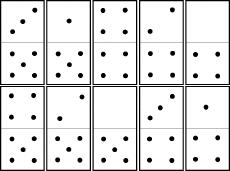
\includegraphics[width=.8\textwidth]{domino.jpg}
\caption{Ako popreklápať kocky domina tak, aby rozdiel medzi 
súčtami horných a dolných políčok bol čo najmenší? }
\label{obr1}
\end{center}
\end{minipage}
\end{center}
\end{figure}

Alebo dva obrázky vedľa seba:

\begin{figure}[ht]
\phantom.\hfill
%
\begin{minipage}{0.4\linewidth}
\begin{center}
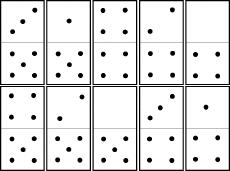
\includegraphics[width=.8\textwidth]{domino.jpg}
\caption{Názov ľavého obrázku}
\label{obrL1}
\end{center}
\end{minipage}
%
\hfill
%
\begin{minipage}{0.4\linewidth}
\begin{center}
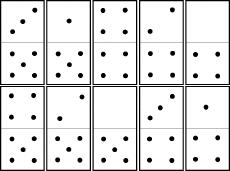
\includegraphics[width=.8\textwidth]{domino.jpg}
\caption{Názov pravého obrázku}
\label{obrP1}
\end{center}
\end{minipage}
%
\hfill\phantom.
\end{figure}



Matematicky možeme vzťahy označiť:

\begin{equation} 
\label{nerov1}
c_{i,j}^2+c_{k,l} \le \frac{c_{i,l}}{c_{k,j}}
\end{equation}

a potom sa naň neskôr v texte~\eqref{nerov1} odvolávať. Ak sa pri reporte objavia symboly 
(??) treba zopakovať \verb|pdflatex praca|.


Môžeme použiť aj iné matematické prostredia:

$$
c_{i,j}^2+c_{k,l} \le \frac{c_{i,l}}{c_{k,j}}
$$

resp.

\begin{displaymath}
c_{i,j}^2+c_{k,l} \le \frac{c_{i,l}}{c_{k,j}}
\end{displaymath}

resp.

\begin{equation*} 
c_{i,j}^2+c_{k,l} \le \frac{c_{i,l}}{c_{k,j}}
\end{equation*}

resp.

\begin{multline*}
c_{i,j}^2+c_{k,l} \le \frac{c_{i,l}}{c_{k,j}} \cdots \mbox{riadok číslo 1} \allowdisplaybreaks\\
c_{i,j}^2+c_{k,l} \le \frac{c_{i,l}}{c_{k,j}} \cdots \mbox{riadok číslo 2} \allowdisplaybreaks\\
c_{i,j}^2+c_{k,l} \le \frac{c_{i,l}}{c_{k,j}} \cdots \mbox{riadok číslo 3} \allowdisplaybreaks\\
c_{i,j}^2+c_{k,l} \le \frac{c_{i,l}}{c_{k,j}} \cdots \mbox{riadok číslo 4}
\end{multline*}

resp.

\begin{multline}
c_{i,j}^2+c_{k,l} \le \frac{c_{i,l}}{c_{k,j}} \cdots \mbox{riadok číslo 1} \\
c_{i,j}^2+c_{k,l} \le \frac{c_{i,l}}{c_{k,j}} \cdots \mbox{riadok číslo 2} \\
c_{i,j}^2+c_{k,l} \le \frac{c_{i,l}}{c_{k,j}} \cdots \mbox{riadok číslo 3} \\
c_{i,j}^2+c_{k,l} \le \frac{c_{i,l}}{c_{k,j}} \cdots \mbox{riadok číslo 4}
\label{vztah-22}
\end{multline}

resp.

\begin{eqnarray*}
c_{i,j}^2+c_{k,l} &\le& \frac{c_{i,l}}{c_{k,j}} \cdots \mbox{riadok číslo 1} \\
c_{i,j}^2+c_{k,l} &\le& \frac{c_{i,l}}{c_{k,j}} \cdots \mbox{riadok číslo 2} \\
c_{i,j}^2+c_{k,l} &\le& \frac{c_{i,l}}{c_{k,j}} \cdots \mbox{riadok číslo 3} \\
c_{i,j}^2+c_{k,l} \le  &xxx& \frac{c_{i,l}}{c_{k,j}} \cdots \mbox{riadok číslo 4}
\end{eqnarray*}

resp.

\begin{eqnarray}
\label{xx01}
c_{i,j}^2+c_{k,l} &\le& \frac{c_{i,l}}{c_{k,j}} \cdots \mbox{riadok číslo 1} \\
\label{xx02}
c_{i,j}^2+c_{k,l} &\le& \frac{c_{i,l}}{c_{k,j}} \cdots \mbox{riadok číslo 2} \\
\label{xx03}\nonumber
c_{i,j}^2+c_{k,l} &\le& \frac{c_{i,l}}{c_{k,j}} \cdots \mbox{riadok číslo 3} \\
\label{xx04}
c_{i,j}^2+c_{k,l} &xxx& \frac{c_{i,l}}{c_{k,j}} \cdots \mbox{riadok číslo 4}
\end{eqnarray}



\noindent
Niekedy sa hodí pracovať s maticami alebo determinantami:

$$
{\mathbb A} = 
\left( \begin{array}{@{}*{3}{r}@{}}
-5 &  8 &  3\\
 0 & -0 &  2\\
 5 &  1 & -2  
\end{array} \right)
%
\times
%
\left[ \begin{array}{@{}*{3}{c}@{}}
-5 &  8 &  3\\
 0 & -0 &  2\\
 5 &  1 & -2  
\end{array} \right\}
%
+
%
\left| \begin{array}{@{}*{3}{r}@{}}
-5 &  8 &  3\\
 0 & -0 &  2\\
 5 &  1 & -2  
\end{array} \right\vert
%
+
%
\left\Vert\begin{array}{@{}*{3}{c}@{}}
-5 & 8,1  & 3,4 \\
x  & -0,2 & 2   \\
5  & 1    & -2  
\end{array} \right\Vert
$$

\begin{figure}[ht]
\begin{center}
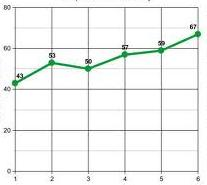
\includegraphics[width=.4\textwidth]{obrazok.jpg}
\caption{Obrázok}
\label{obr2}
\end{center}
\end{figure}

Tu je potrebné popísať doteraz získané poznatky z problematiky. 
Nezabudnúť dôsledne citovať autorov článkov, kníh aj internetových publikácií 
napr. monografia \cite{pes2, berman}. 

Na obrázku \ref{obr1a} máme príklad zo zábavnej matematiky uvedený v práci Peško \cite{pes2}.
Porovnajte definíciu, zobrazenie a tiež umiestnenie obrázku \ref{obr1a} s obrázkom \ref{obr1}.

\begin{figure}[ht]
\begin{center}
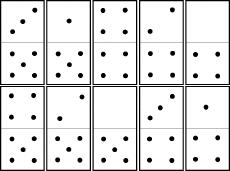
\includegraphics[width=.5\textwidth]{domino.jpg}
\caption{Ako popreklápať kocky domina tak, aby rozdiel medzi 
súčtami horných a dolných políčok bol čo najmenší? }
\label{obr1a}
\end{center}
\end{figure}

	%  Súčasný stav
\chapter{Matematický model}

Tu je vhodné uviesť ďalej používané základné pojmy a tvrdenia. 
Čitetel ocení ak sú tieto demonštrované na výstižných ilustračných príkladoch. 
Opäť nezabudnúť dôsledne citovať autorov. 
U vlastných výsledov sa zse nehambiť na túto skutočnosť upozorniť -- napríklad názvom podkapitoly.


\section{Problém pažravej trojhodnotovej stonožky}

Nech $m,n,a,b$ prirodzené čísla $n,m \ge 2$ a $0<a<b$. 
Sú dané $n$-tice prirodzených čísel ${\mathrm a}=(a_1,\dots,a_j,\dots,a_n)$
a ${\mathrm b}=(b_1,\dots,b_j,\dots,b_n)$ také, že $a_j+b_j \le m$.
Hľadá sa taká matica ${\mathrm A}=(a_{ij})_{m\times n}$, ktorá v každom
stĺpci $j$ obsahuje aspoň $a_j$ prvkov rovných $a$ a aspoň $b_j$ prvkov rovných $b$,
pričom rozdiel medzi najväčším a najmenším  riadkovým súčtom prvkov matice ${\mathrm A}$ 
je čo najmenší.

Označme $M=\{1,2,\dots,m\}$ a $N=\{1,2,\dots,n\}$. 
Uvažujme premenné matice 
${\mathrm X} = (x_{ij})_{m\times n}$, ${\mathrm Y}=(y_{ij})_{m\times n}$ s prvkami

$$
x_{ij}=\left\{\begin{array}{ll}
	 1, &\mbox{ak } a_{ij}=a \\
	 0, &\text{inak}         \end{array}\right.
\quad 
y_{ij}=\Bigg\{\bigg\{\Big\{\big\{\begin{array}{ll}
	 1, &\mbox{ak } a_{ij}=b \\
	 0, &\mbox{inak}.        \end{array}
\quad 
y_{ij}=\Big\{\begin{array}{ll}
	 1, &\mbox{ak } a_{ij}=b \\[-.5em]
	 0, &\mbox{inak}.        \end{array}
$$

Zátvorka \verb|\left\{| musí mať pravý pár,  napr. \verb|\right\}|  alebo,  ak nechceme mať na
druhej strane nič, použijeme príkaz s bodkou \verb|\right.|

Nech $m,n,a,b$ prirodzené čísla $n,m \ge 2$ a $0<a<b$. 
Sú dané $n$-tice prirodzených čísel ${\mathrm a}=(a_1,\dots,a_j,\dots,a_n)$
a ${\mathrm b}=(b_1,\dots,b_j,\dots,b_n)$ také, že $a_j+b_j \le m$.
Hľadá sa taká matica ${\mathrm A}=(a_{ij})_{m\times n}$, ktorá v každom
stĺpci $j$ obsahuje aspoň $a_j$ prvkov rovných $a$ a aspoň $b_j$ prvkov rovných $b$,
pričom rozdiel medzi najväčším a najmenším  riadkovým súčtom prvkov matice ${\mathrm A}$ 
je čo najmenší.



Problém možno riešiť ako nasledujúcu úlohu matematického programovania:

\begin{alignat}{2} \label{u_1}
& z_2-z_1 \rightarrow \min             &                  &             \\
& \sum_{i\in M} x_{ij} \ge a_j,        &j\in N,           & \label{u_2} \\
& \sum_{i\in M} y_{ij} \ge b_j,        &j\in N,           & \label{u_3} \\
& x_{ij} + y_{ij} \le 1,               &i\in M, j\in N,   & \label{u_4} \\
& \sum_{i\in M} x_{ij}+ y_{ij} \le m,  &j\in N,           & \label{u_5} \\
& z_1 \le \sum_{j\in N} a\cdot x_{ij}+b\cdot y_{ij} \le z_2,  
                                       &i\in M,           & \label{u_6} \\
& x_{ij}, y_{ij} \in \{0,1\},          &i\in M, j\in N,   & \label{u_7} \\
& z_1, z_2 \ge 0.                      &                  & \label{u_8}
\end{alignat}

alebo ináč usporiadané a niektoré sumy ináč zobrazené:

\begin{alignat}{2} \label{u_1}
& z_2-z_1 \rightarrow \min             &&                               \allowdisplaybreaks\\
& \sum_{i\in M} x_{ij} \ge a_j,        &&j\in N,            \label{v_2} \allowdisplaybreaks\\
&\textstyle \sum_{i\in M} x_{ij} \ge a_j,          
                                       &&j\in N,            \nonumber   \allowdisplaybreaks\\
&\textstyle \sum\limits_{i\in M} x_{ij} \ge a_j,
                                       &&j\in N,            \nonumber   \allowdisplaybreaks\\
& \sum_{i\in M} y_{ij} \ge b_j,        &&j\in N,            \label{v_3} \allowdisplaybreaks\\
& x_{ij} + y_{ij} \le 1,               &&i\in M, j\in N,    \label{v_4} \allowdisplaybreaks\\
& \sum_{i\in M} x_{ij}+ y_{ij} \le m,  &&j\in N,            \label{v_5} \allowdisplaybreaks\\
z_1 \le &\sum_{j\in N} a\cdot x_{ij}+b\cdot y_{ij} \le z_2,\qquad  
                                       &&i\in M,            \label{v_6} \allowdisplaybreaks\\
& x_{ij}, y_{ij} \in \{0,1\},          &&i\in M, j\in N,    \label{v_7} \allowdisplaybreaks\\
& z_1, z_2 \ge 0.                      &&                   \label{v_8}
\end{alignat}



Jednotkové hodnoty premenných $x_{ij}$ resp. $y_{ij}$ zodpovedajú umiestneniu
hodnoty $a$ resp. $b$ v $i$-tom riadku a v $j$-tom stĺpci hľadanej matice.
Optimálnym riešením je potom matica ${\mathrm A} = (a_{ij})_{m\times n}$  s prvkami
%
$$ a_{ij} = a\cdot x_{ij}+b\cdot y_{ij}.$$

V cieľovej funkcii~\eqref{u_1} je hodnota premennej $z_2$ rovná najväčšiemu
riadkovému súčtu prvkov matice a hodnota premennej $z_1$ zas najmenšiemu
riadkovému súčtu. Podmienky~\eqref{u_2} a~\eqref{u_3} zabezpečujú, že bude
vybraných najmenej $a_j$ hodnôt $a$ a najmenej $b_j$ hodnôt $b$ v každom
stĺpci $j$. 
Podmienka~\eqref{u_4} zabráni umiestneniu oboch nenulových hodnôt
$a,b$ do jediného prvku $a_{ij}$ matice. 
Podmienka~\eqref{u_5}
obmedzuje zhora celkový počet nenulových prvkov v každom stĺpci počtom $m$
-- riadkov matice. Podmienkou~\eqref{u_6}
sú definované horná $z_2$ a dolná $z_1$ hranica riadkových súčtov. 
Obmedzenia premených~\eqref{u_7} a~\eqref{u_8} sú obligatorné.



	%  Matematický model
\chapter{Metódy riešenia}

Tu treba výstižne popísať zvolené metódy riešenia. Aj je to možné porovnať ich teoreticky.
Tu sú uvedené dva príklady listingov:

\begin{lstlisting}[mathescape]{}
procedure FLOYD(${\mathrm A}$)
  ${\mathrm D} = {\mathrm A}$
  for $k \in N$ do 
    for $i \in N$ do 
      for $j \in N$ do
        if $d_{ij} > d_{ik}+d_{kj}$ then
           $d_{ij} = d_{ik}+d_{kj}$
$\text{return}~{\mathrm D}$
\end{lstlisting}


\hrule

\lstset{%
language={[Sharp]C},
breaklines=true,
breakindent=0pt,
tabsize=2,
showstringspaces=true
}
%
\begin{lstlisting}
using System;
public class Foo
{
 public static void Main()
 {
     Console.WriteLine("I Love LaTeX");//This is a comment.
 }
 /*This is a comment too.*/
}
\end{lstlisting}



	%  Metódy riešenie
\chapter{Počítačové experimenty}

Tu treba popísať a vyhodnotiť výsledky počítačových experimentov.





	%  Počítačové experimenty
\chapter{Záver}

Tu treba zhodnotiť dosiahnuté výsledy a načrtnúť dalšie možné cesty riešenia.



	%  Zaver


%%%%%%%%%%%%%%%%%% literatura


%%%%%%%%%%%%%%%%%%%%%%%%%%%%%%%%%%%%%%%%%%%%%%%%%%%%%%%%%%%%%%%%%%%%%%%%%%%%%
\begin{thebibliography}{99}                                \label{literatura}
%\addcontentsline{toc}{section}{Literatúra}
\addcontentsline{toc}{chapter}{Literatúra}

\bibitem{root_arm}
Mikroprocesory s architekturou ARM
\url{http://www.root.cz/clanky/mikroprocesory-s-architekturou-arm/}

\bibitem{msp430_mcu}
Popis mikrokontroléra msp430
\url{www.ti.com/lit/ug/slau049f/slau049f.pdf}

\bibitem{arm_list}
zoznam ARM jadier
\url{http://en.wikipedia.org/wiki/List_of_ARM_microprocessor_cores}

\bibitem{68HC11}
jadro 68HC11
\url{http://www.clear.rice.edu/elec201/Book/6811_asm.html}


\bibitem{inside_cortex}
inside Cortex príručka
\url{http://www.hitex.com/fileadmin/pdf/insiders-guides/stm32/isg-stm32-v18d-scr.pdf}



\bibitem{context_switch}
prepínanie kontextu
\url{http://www.eetimes.com/General/PrintView/4370755}

\bibitem{operacni_systemi}
Doc. Ing. František Plášil, CSc., Doc. Ing. Jan Staudek, CSc., 
{\it Operační systémi}, 
Knižnice výpočetní techniky, 
Nakladatelství technické literatury (1992), 
SNTL, ISBN 80-03-00269-9.


\bibitem{linux_gui}
zoznam grafických rozhraní
\url{http://www.cyberciti.biz/faq/does-the-unix-or-linux-has-gui/}

\bibitem{ti_msp430}
nízkospotrebná rada mcu msp430
\url{http://www.ti.com/lsds/ti/microcontroller/16-bit_msp430/overview.page?DCMP=MCU_other&HQS=msp430}

\bibitem{qp_project}
platforma qp
\url{http://www.state-machine.com/}

\bibitem{android_event} 
udalosťami riadené programovanie na Androide
\url{http://independentlyemployed.co.uk/2010/12/03/android-event-driven-programming/}

\bibitem{apollo_agc} 
navigačný počítač lode Apollo
\url{http://www.apolloguidancecomputer.com/}


\bibitem{rom_fs} 
súborový systém romfs
\url{http://romfs.sourceforge.net/}


\bibitem{discovery_kit} 
vývojová doska Stm32 Discovery
\url{http://www.st.com/web/catalog/tools/FM116/SC959/SS1532/PF250863}

\bibitem{usb_uart} 
prevodník usb na uart
\url{http://www.ftdichip.com/Products/ICs/FT232BM.htm}

\bibitem{stellaris_kit} 
vývojová doska Stellaris Launchpad
\url{http://www.ti.com/tool/ek-lm4f120xl}




\bibitem{arm_summom_git} 
summon arm toolchain
\url{https://github.com/esden/summon-arm-toolchain}

\bibitem{stlink} 
nástroj stlink flash
\url{https://github.com/texane/stlink}

\bibitem{lm4_flash} 
nástroj lm4 flash
\url{https://github.com/utzig/lm4tools/tree/master/lm4flash}

\bibitem{stellaris_ware} 
knižnica Stellarisware
\url{http://www.ti.com/tool/sw-grl}

\bibitem{suzuha_source} 
zdrojové súbory operačného systému
\url{http://sourceforge.net/projects/suzuhaos/files/}


\end{thebibliography}
	%  Literatura

\end{document}


